% !TEX root=MemoriaTFG.tex

\chapter{Switch-PC interface}
A key aspect to the project consist in how we connect the \ac{PC} and the console. The first part of it, getting the images from the game, has already been dealt with in the previous chapter, but now comes the challenging part. We need to somehow make the neural net's output get to the console.

\section{Approaches and final solution}
As mentioned in the introduction, there is no way to control the Nintendo switch besides using its own controller. The first thing that came to mind was building a robot capable of pressing the buttons itself whenever we told it to. A rough way of implementing it was thought about and some actual piece candidates where found, but nothing came of it, as the difficulty of building such device could be a final project of its own.

Parallely, a way of faking the pc as a controller was investigated. A project that could record input onto an arduino and then send it to the switch by connecting it directly into the console's controller port, was found, which told us that accessing the console was possible. This works by using the same checking protocol sequence as a Nintendo controller when trying to connect the device.

By modifying the project, we allowed for it to instead of record some input sequence, receive it from the PC. As the project comes with a python script that contains the whole controller scheme and methods to test and ensure a good connection, we can plug the script directly in our project for its future use.

\section{Arduino tools}
The original project only used the arduino seen in image \ref{arduino}, which already had the commands imprinted in a loop. This time around, as it is connected to our \ac{PC} using a USB-TTL converter (\ref{appendix:USBTOTTL}), seen in \ref{USBtoTTL}, the loop waits for the input and sends it to the console.

The USB-TTL converter must be connected according to the information given by the own device, which means that contrary to what is most common, RX to TX and TX to RX, it is done backwards. This is only because the converter tells us where the connection must go and not what it actually is. As for the ground and 5V cables there is no room for doubt.

\begin{figure}[h]
\centering
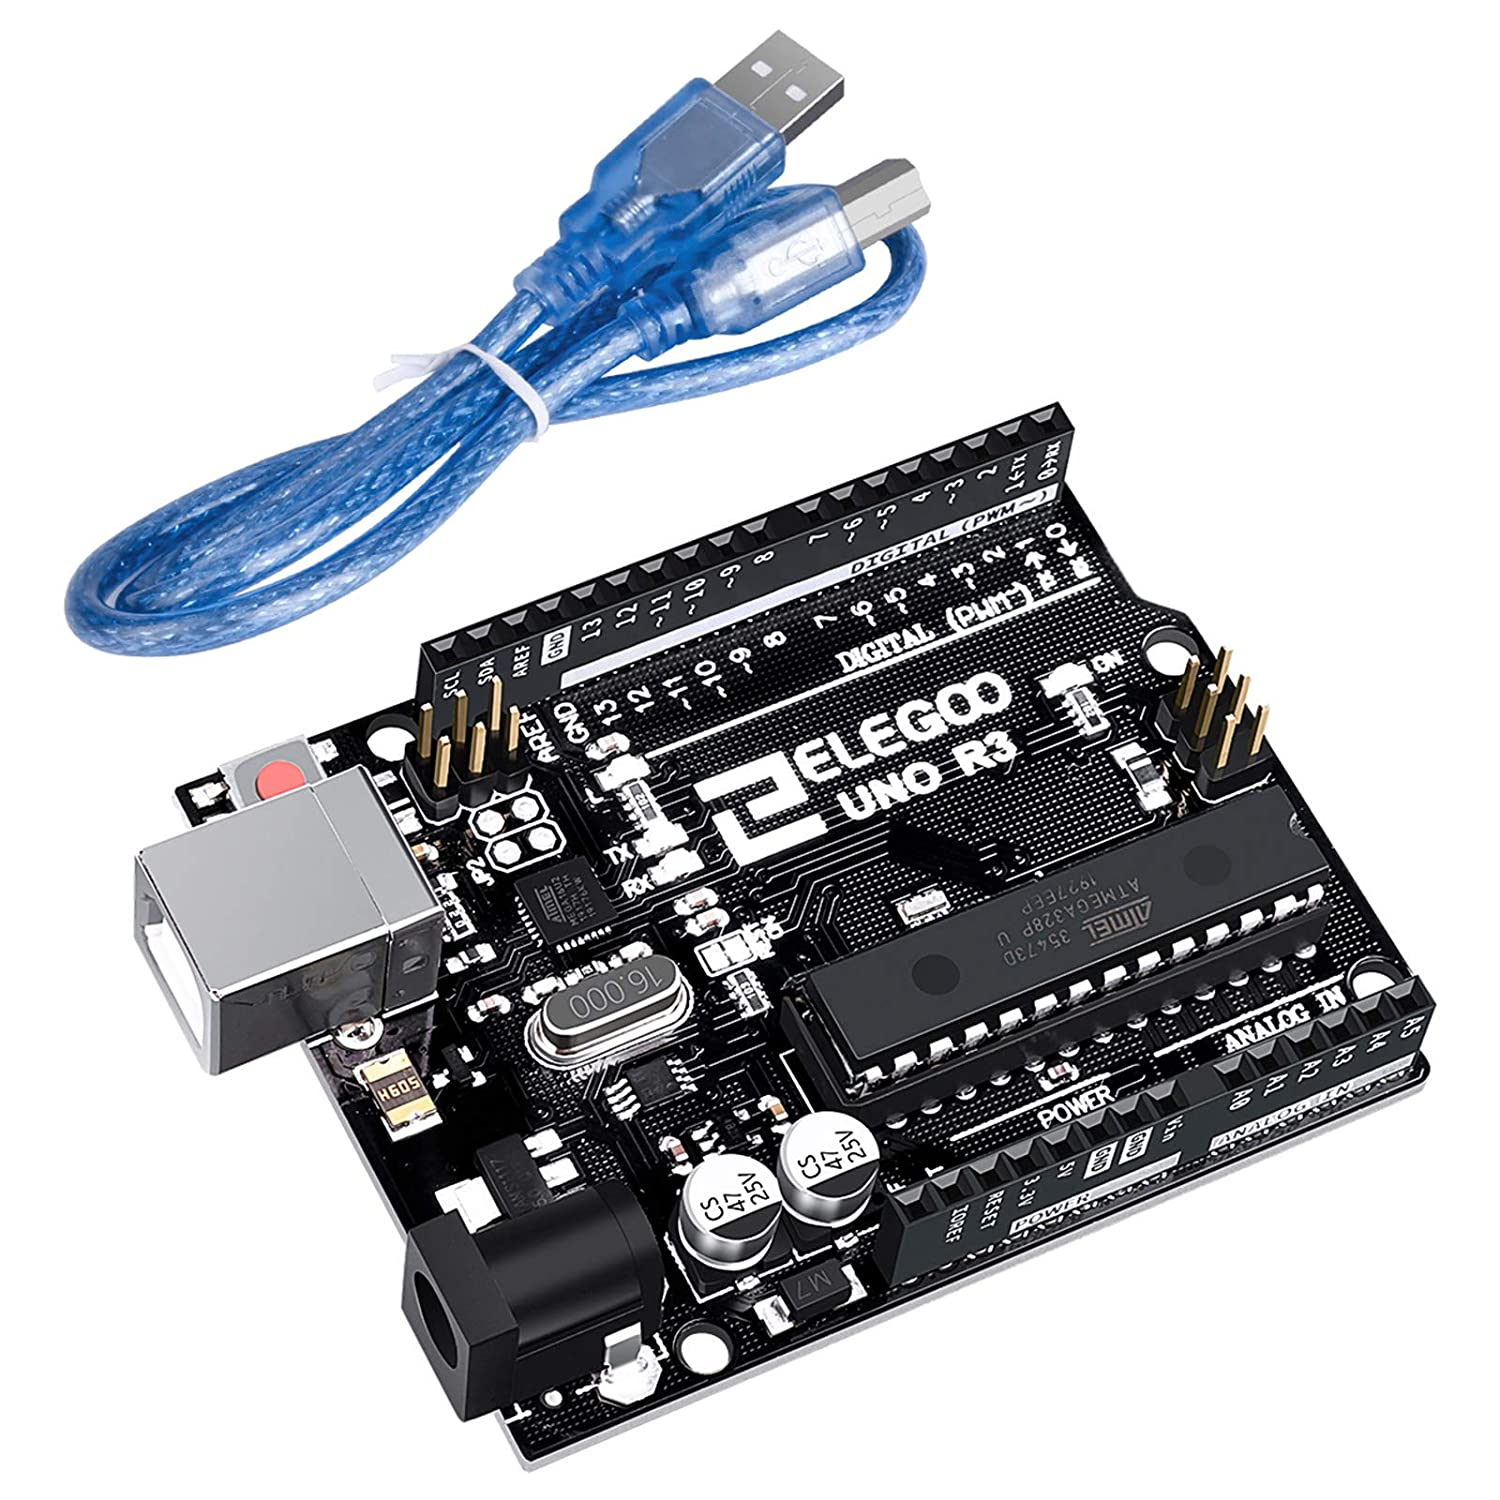
\includegraphics[width=.4\linewidth]{image024}
\caption{\label{arduino}Arduino ELEGOO UNO R3}
\end{figure}
\begin{figure}[h]

\centering
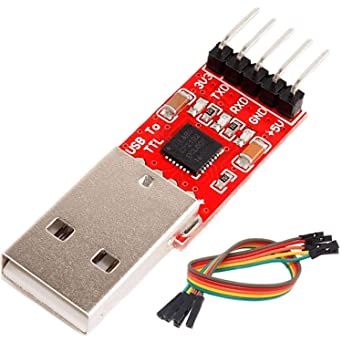
\includegraphics[width=.4\linewidth]{image025}
\caption{\label{USBtoTTL}USB to TTL CP2102}
\end{figure}